\documentclass{article}

% if you need to pass options to natbib, use, e.g.:
%     \PassOptionsToPackage{numbers, compress}{natbib}
% before loading neurips_2020

% ready for submission
% \usepackage{neurips_2020}

% to compile a preprint version, e.g., for submission to arXiv, add add the
% [preprint] option:
%     \usepackage[preprint]{neurips_2020}

% to compile a camera-ready version, add the [final] option, e.g.:
%     \usepackage[final]{neurips_2020}

% to avoid loading the natbib package, add option nonatbib:
     \usepackage[final]{neurips_2020}

\usepackage[utf8]{inputenc} % allow utf-8 input
\usepackage[T1]{fontenc}    % use 8-bit T1 fonts
\usepackage{hyperref}       % hyperlinks
\usepackage{url}            % simple URL typesetting
\usepackage{booktabs}       % professional-quality tables
\usepackage{amsfonts}       % blackboard math symbols
\usepackage{nicefrac}       % compact symbols for 1/2, etc.
\usepackage{microtype}      % microtypography

\usepackage{amsmath,amsthm,amssymb}
\usepackage{graphicx}
\usepackage{mathtools}
\usepackage{multicol}
\usepackage{float}

% URL Stuff
\hypersetup{
colorlinks=true,
linkcolor=blue,
filecolor=magenta,
urlcolor=cyan,
}

% Math stuff
\DeclarePairedDelimiter{\ceil}{\lceil}{\rceil}
\DeclarePairedDelimiter\floor{\lfloor}{\rfloor}

% Image stuff
\graphicspath{ {.} }



\title{Comparing the interpretability of GAN architectures}

% The \author macro works with any number of authors. There are two commands
% used to separate the names and addresses of multiple authors: \And and \AND.
%
% Using \And between authors leaves it to LaTeX to determine where to break the
% lines. Using \AND forces a line break at that point. So, if LaTeX puts 3 of 4
% authors names on the first line, and the last on the second line, try using
% \AND instead of \And before the third author name.

\author{%
  Henry Tu \\
  Department of Computer Science\\
  University of Toronto\\
  Toronto, ON M5S 1A1 \\
  \texttt{henry.tu@mail.utoronto.ca} \\
  % examples of more authors
   \And
     Seel Patel \\
  Department of Computer Science\\
  University of Toronto\\
  Toronto, ON M5S 1A1 \\
  \texttt{seel.patel@mail.utoronto.ca} \\
  % \AND
  % Coauthor \\
  % Affiliation \\
  % Address \\
  % \texttt{email} \\
  % \And
  % Coauthor \\
  % Affiliation \\
  % Address \\
  % \texttt{email} \\
  % \And
  % Coauthor \\
  % Affiliation \\
  % Address \\
  % \texttt{email} \\
}

\begin{document}

\maketitle

\begin{abstract}
  A Generative Adversarial Network (GAN) uses an adversarial process between two models which are simultaneously trained to estimate a generative model.\cite{gan}
        There are many architectures, such as COCO-GAN\cite{cocogan} and StyleGAN\cite{stylegan}, which can generate samples that mimic real images.
        We are exploring methods of comparing the quantitative performance of these architectures with their interpretability.
        Our quantitative measures include C2ST\cite{evaluateGANs} and image quality measures\cite{evaluateGANs}.
        To analyze these networks qualitatively, we will use methods such as Latent Space Exploration\cite{sampleGAN} and nearest neighbour tests\cite{evaluateGANs} to decipher what the networks have learned.
        By combining these two forms of analysis, we will gain insight into the relationship between performance metrics and the generated output of the models.
\end{abstract}

\section{Introduction}

 StyleGAN and COCO-GAN generate images using different techniques to accomplish two different goals: StyleGAN is designed such that high level features of the output image can be finely tuned and adjusted (e.g. lighting, hair colour, etc.)\cite{stylegan}.
        On the other hand, COCO-GAN generates each part of the image separately before stitching it together in order to simulate the human perception of vision\cite{cocogan}.
        As a result, we expected each model to generate images with different qualities that relate to their designed tasks.
        Both GAN models were trained on the LSUN Bedroom dataset\cite{lsunBedroom} at a resolution of $256 \times 256$.
        Due to time constraints, we used pre-trained models to generate images for our analysis.
        \\\\
        NVIDIA Research Projects' Official TensorFlow Implementation of StyleGAN pretrained to the LSUN Bedroom dataset\cite{styleGANCode} was used with
        5000 latent vectors $\mathbf{z} \in \mathbb{R}^{512} \sim \mathcal{N}(0, 1\mathbf{I})$, which each correspond to an output image.
        The TensorFlow implementation of COCO-GAN by its authors pretrained to the LSUN Bedroom dataset\cite{cocogan} using
        5000 latent vectors $\mathbf{z} \in [-1, 1]^{128} \sim \mathcal{U}[-1, 1]^{128}$, which each correspond to an output image. 


        \section{Quantitative analysis}
        \label{sec:quantitative}
        \subsection{Classifier Two-Sample tests (C2ST)}
        \label{subsec:c2st}
        C2ST is used to predict if two samples came from the same distribution\cite{c2st}.
        We trained a CNN to perform classification using a variation of the DCGAN discriminator\cite{dcgan}.
        The goal is to compare the difficulty in which the classifier has with distinguishing between real and generated samples.
        The classifier was trained using Cross Entropy loss and the Adam optimizer.
        \begin{figure}[!htb]
          \centering
          \includegraphics[scale=0.3]{c2st-diagram.png}\\
          \caption{ \textbf{C2ST architecture.} For all Conv2D layers, Kernel Size: 3, Stride: 2, Padding: 1, Leaky ReLU slope: 0.2. Let $\mathbf{f}: [0, 1]^{3 \times 256 \times 256} \rightarrow \mathbb{R}^{2}$ be the neural network. Let $GANImages, RealImages \in [0, 1]^{3 \times 256 \times 256}$ be the distribution of generated images and samples from the LSUN bedroom dataset respectively. For $\mathbf{x}_{real} \sim RealImages$ (Class 1) and $\mathbf{x}_{gan} \sim GANImages$ (Class 0), the predicted class $\hat{c} =argmax_c (\mathbf{f}(\mathbf{x})[c])$ is correct iff $\hat{c} = class(\mathbf{x})$.}
        \end{figure}
        The training, validation, and test datasets were drawn from $\beta RealImages + (1 - \beta)GANImages, \beta \sim Bern(0.5)$.
        Out of the pool of 10000 images, 5000 were allocated for training, 2500 validation, and 2500 testing.
        Let $StyleGANImages, COCOGANImages$ be the distribution of StyleGAN and COCO-GAN generated images respectively. The model was trained with a batch size of 200 for 1000 epoches. Let $GANImages = \beta StyleGANImages + (1 - \beta) COCOGANImages, \beta \sim Bern(0.5)$.
        After tuning hyper parameters and performing early stopping, the following results were attained:
        
        \begin{figure}[H]
            \centering
            \begin{tabular}{ |p{3cm}|p{2cm}|  }
                 \hline
                 \multicolumn{2}{|c|}{Table 1: Real vs GAN classifier} \\
                 \hline
                Data Set     & Accuracy\\
                 \hline
                Training        & 75.9\% of 5000 \\
                 \hline
                Validation      & 67.6\% of 2500 \\
                 \hline
                Test (Real)     & 58.2\% of 1250 \\
                 \hline
                Test (StyleGAN) & 60.5\% of 625  \\
                 \hline
                Test (COCO-GAN) & 89.6\% of 625 \\
                 \hline 
            \end{tabular}
        \end{figure}
        
        This data suggests that StyleGAN is better at tricking the classifier than COCO-GAN.
        To confirm this, we trained additional classifiers using images from only one of the GAN models. Let $GANImages = StyleGANImages, COCOGANImages$ respectively:

        \begin{multicols}{2}
            \begin{tabular}{ |p{3cm}|p{2cm}|  }
                 \hline
                 \multicolumn{2}{|c|}{Table 2: Real vs StyleGAN classifier} \\
                 \hline
                Data Set     & Accuracy\\
                 \hline
                Training        & 77.6\% of 5000 \\
                 \hline
                Validation      & 68.1\% of 2500 \\
                 \hline
                Test (Real)     & 74.6\% of 1250 \\
                 \hline
                Test (StyleGAN) & 61.4\% of 1250  \\
                 \hline
            \end{tabular}
        
            \begin{tabular}{ |p{3cm}|p{2cm}|  }
                 \hline
                 \multicolumn{2}{|c|}{Table 3: Real vs COCO-GAN classifier} \\
                 \hline
                Data Set     & Accuracy\\
                 \hline
                Training        & 87.9\% of 5000 \\
                 \hline
                Validation      & 88.2\% of 2500 \\
                 \hline
                Test (Real)     & 96.4\% of 1250 \\
                 \hline
                Test (COCO-GAN) & 76.1\% of 1250 \\
                 \hline
            \end{tabular}
        \end{multicols}
            
        As seen here, the Real vs COCO-GAN classifier (Table 3) performed significantly better than the Real vs StyleGAN classifier (Table 2).
        \subsection{Image sharpness}
        \label{subsec:imageSharpness}
        A common indicator of image quality is sharpness.
        When an image is sharp, the details within the image are seen more clearly and there is a better distinction between different objects in the picture.
        Overall, this allows humans to form a better understanding of what they are seeing when they view the image.
        Using directional image gradients along the $x$ and $y$ axes, we measured the mean image sharpness of the generated images and real images as seen below. (Higher is better)
        
        \begin{figure}[H]
            \centering
            \begin{tabular}{ |p{2cm}|p{2cm}|p{2cm}|p{2cm}|  }
                 \hline
                 \multicolumn{4}{|c|}{Table 4: Mean image sharpness} \\
                 \hline
                & Real & StyleGAN & COCO-GAN  \\
                \hline
                Sharpness & 8.534    & 8.214      & 7.970\\
                \hline
            \end{tabular}
        \end{figure}
        
        Therefore the real images are the sharpest and StyleGAN does the better job of producing sharper images than COCO-GAN.
        However, does higher sharpness always mean better image quality?
        We explore this question in the combined analysis section below.

        \subsection{Color distribution comparison}
        \label{subsec:colorDistribution}
        In order to properly mimic the real images, the generated images have to closely follow the color distribution of the real images. Each image is represented by RGB values between 0 and 1. We extracted the frequencies of RGB color values using 25 bins for each of the datasets. The distributions of these frequencies are plotted in the appendix for the real and generated images. 
        %\\ \\
        % \\
        % \includegraphics[scale =0.3]{color-distributions/real_color_freq.png} \\
        % \includegraphics[scale =0.3]{color-distributions/stylegan_color_freq.png} \\
        % \includegraphics[scale =0.3]{color-distributions/cocogan_color_freq.png} \\
        % \\
        From the frequency plots, we see that both models do a good job of matching the real distribution of colors.
        However, both generated image color frequency plots show many spikes that are not present in the real image frequency plot.
        We will explore these spikes in our combined analysis section. Additionally, to quantify this color reproduction quality, we also took the KL Divergence between the generated image color distributions to the real images.
        
        \begin{figure}[H]
            \centering
            \begin{tabular}{ |p{2cm}|p{1cm}|p{1cm}|p{1cm}|p{1cm}|  }
                 \hline
                 \multicolumn{5}{|c|}{Table 5: KL divergence of color channels w/ real imgs} \\
                 \hline
                & Red & Green & Blue & Gray  \\
                \hline
                StyleGAN & 0.286    & 0.263      & 0.232     &  0.251 \\
                \hline
                COCO-GAN  & 0.044    & 0.047      & 0.059     &  0.016\\
                \hline
            \end{tabular}
        \end{figure}
        
        Therefore COCO-GAN does a statistically better job of modelling the color distribution of the real images. Note that this does not guarantee that COCO-GAN is superior because this method of comparison does not take into account the spatial position of the colors. This means that the images would post the same KL Divergence even if the pixels were scrambled. Therefore further analysis is needed to determine which model performs better overall.
        \section{Qualitative analysis}
        \label{sec:qualitative}
        % \subsection{Latent space exploration}
        % \label{subsec:latentSpaceExploration}
        % An important part of the generator is it's ability to combine different features from the real image in order to generate new images.
        % For example, in our dataset, an image could contain a bed, a window or a painting. What about a combination of these?
        % What if the locations of these features is changed? We use latent space interpolation to determine if the model produces robust images in all of these cases.
        \subsection{Nearest neighbours}
        \label{subsec:nearestneighbours}
        A common problem within GANs is mode collapse.
        This occurs when the generator consistently outputs the same image for distinct latent vectors.
        In addition to this, we want to identify if the generator creates multiple images with identical structure or color scheme.
        To identify these issues, we randomly sampled generated images and visually compared them with the k nearest neighbours from the images produced by the same model.
        In our search, we found no evidence of mode collapse in either StyleGAN or COCO-GAN. View the appendix for samples used in the analysis.
        \section{Combined analysis}
        \label{sec:combinedAnalysis}
        
        \subsection{Colour frequency peaks}
        In our analysis of color frequency distributions above, we noticed that both StyleGAN and COCO-GAN exhibited spikes in their frequency graphs.
        For both models, one prominent spike occurs simultaneously in the green and blue channel at intensity level 0.6.
        % %
        % \\\begin{figure}[!htb]
        %   \centering
        %   \includegraphics[scale=0.1]{gradient.png} 
        %   \caption{ (0,0.6,0.6)$\longrightarrow$(1.0,0.6,0.6) RGB gradient}
        % \end{figure} \\
        % %
        We decided to sample some of these colors and found generated images with color schemes closely matching them.
        %
        
        \begin{figure}[H]
          \centering
          \includegraphics[scale=0.28]{color-images/03_06_06_stylegan_images.png} 
          \includegraphics[scale=0.28]{color-images/03_06_06_coco_images.png}
          \caption{\textbf{RGB (0.3,0.6,0.6) StyleGAN images vs CocoGAN images.}
            For both models, we are seeing an increase in noise and distortion in the images.
            Especially COCO-GAN,  which displays noisy textures or bad structure in every image.
            What does this trend tell us about COCO-GAN?
            From the samples, we can see that many of these images have windows in them that display the sky.
            COCO-GAN has done a relatively poor job of displaying the sky and natural imagery in the background.
            Additionally, in the COCO-GAN images the sky color often bleeds into the rest of the image and takes on colors from our gradient of interest.
            Therefore we theorize that this spike in frequency occurs from COCO-GAN's inability to generate good images that include the sky.
        }
        \end{figure}
        
        \subsection{High sharpness images}
        In our image sharpness analysis, we found that StyleGAN produced sharper images than COCO-GAN.
        To qualitatively explore this higher sharpness, we plotted the sharpest images from both models.
         %
        \begin{figure}[H]
          \centering
          \includegraphics[scale=0.25]{sharpness-images/stylegan_sharpness.png} 
          \ \ 
          \includegraphics[scale=0.25]{sharpness-images/coco_sharpness.png}
          \caption{\textbf{Sharpest StyleGAN images vs sharpest COCO-GAN images.} As we can see, the StyleGAN images are of high quality, but the COCO-GAN images are consistently filled with noisy patterns.
            Both sets consist of very sharp images, and therefore we have visualized the sharpness of these images below in order to understand why there is such a large difference in quality.\\}
        \includegraphics[scale=0.25]{sharpness-images/stylegan_sharpness_lines.png}
          \ \
          \includegraphics[scale=0.25]{sharpness-images/coco_sharpness_lines.png}
          \caption{\textbf{StyleGAN vs COCO-GAN sharpness visualizations.} We can see that the sharpness of StyleGAN comes from effectively generating complex patterns while the sharpness of CocoGAN comes from unwanted noise and messy patterns. Therefore, the qualitative analysis indicates that the quality of CocoGAN images is lower than sharpness numbers indicate.}
        \end{figure} 
        %
        %
        \subsection{C2ST smoothgrad analysis}
        We can use SmoothGrad to generate a sensitivity map to visually discover which parts of the image most strongly affects the classification \cite{smoothgrad}.
        Smoothgrad was performed on all 3 classifier models outlined in the C2ST section from earlier. 
        Let $\mathbf{x} \in [0, 1]^{3 \times 256 \times 256}$ be the input image, $\mathcal{L}$ be CE loss, and $\nabla_{\mathbf{x}}^{*} \mathcal{L} (\mathbf{x})$ be the sensitivity map. $\nabla_{\mathbf{x}}^{*} \mathcal{L} (\mathbf{x}) = \frac{1}{100} \sum_{i=1}^{100} \nabla_{\mathbf{x}} \mathcal{L} (\mathbf{x} + \mathcal{N}(0, 0.1^2\mathbf{I}))$. 
        Additional sensitivity map samples are available in the appendix.
        
        \begin{figure}[H]
          \centering
          1
          \includegraphics[scale=0.25]{smoothgrad/combined/real.png}
          2
          \includegraphics[scale=0.25]{smoothgrad/combined/stylegan.png}
          3
          \includegraphics[scale=0.25]{smoothgrad/combined/coco.png}
          \caption{\textbf{Real vs GAN classifier sensitivity map. (1: real, 2: StyleGAN, 3: COCO-GAN)} Evidently, there is a clear checkerboard pattern, which could be caused by COCO-GAN's tile generation\cite{cocogan}. 
        We can use the classifier trained on only one GAN to validate this theory.\\}
            1
            \includegraphics[scale=0.25]{smoothgrad/stylegan/real.png}
            2
            \includegraphics[scale=0.25]{smoothgrad/stylegan/stylegan.png}
            3
            \includegraphics[scale=0.25]{smoothgrad/coco/real.png}
            4
            \includegraphics[scale=0.25]{smoothgrad/coco/coco.png}
          \caption{\textbf{Real vs StyleGAN $\{1, 2\}$ \& Real vs COCO-GAN $\{3, 4\}$ classifier sensitivity map.} $\{1, 3\}$ are real images, and $\{2, 4\}$ are from StyleGAN and COCO-GAN respectively. As seen in images $\{3, 4\}$, the Real vs COCO-GAN classifier uses a checkerboard filter, which is quite effective with a test accuracy of $\frac{76.1\% + 96.4\%}{2} = 86.3\%$ (Table 3). 
          On the other hand, the StyleGAN classifier (images $\{1, 2\}$) is very uniform and shows very few artifacts.
        This seems to suggest there are irregularities in between tiles generated by COCO-GAN which are easily detected by the classifier.
        Therefore according to C2ST, StyleGAN produces more realistic images than COCO-GAN.}
        \end{figure}
        
        \section{Conclusion}
        In conclusion, ...
        
        
\newpage
\begin{thebibliography}{9}
        \bibitem{gan}
        Ian J. Goodfellow, Jean Pouget-Abadie, Mehdi Mirza, Bing Xu, David Warde-Farley, Sherjil Ozair, Aaron Courville, and Yoshua Bengio. (2014)
        \href{https://papers.nips.cc/paper/2014/file/5ca3e9b122f61f8f06494c97b1afccf3-Paper.pdf}{\textit{Generative Adversarial Networks} }

        \bibitem{cocogan}
        Chieh Hubert Lin, Chia-Che Chang, Yu-Sheng Chen, Da-Cheng Juan, Wei Wei, Hwann-Tzong Chen. (2019)
        \href{https://arxiv.org/pdf/1904.00284.pdf}{\textit{COCO-GAN: Generation by Parts via Conditional Coordinating} }

        \bibitem{stylegan}
        Tero Karras, Samuli Laine, Timo Aila. (2018)
        \href{https://arxiv.org/pdf/1812.04948.pdf}{\textit{A Style-Based Generator Architecture for Generative Adversarial Networks} }

        \bibitem{evaluateGANs}
        Brownlee, Jason. (2019)
        \href{https://machinelearningmastery.com/how-to-evaluate-generative-adversarial-networks/}{\textit{How to Evaluate Generative Adversarial Networks}}

        \bibitem{sampleGAN}
        Tom White. (2016)
        \href{https://arxiv.org/pdf/1609.04468.pdf}{\textit{Sampling Generative Networks} }

        \bibitem{lsunBedroom}
        Yu, Fisher and Zhang, Yinda and Song, Shuran and Seff, Ari and Xiao, Jianxiong. (2015)
        \href{https://arxiv.org/pdf/1506.03365.pdf}{\textit{LSUN: Construction of a Large-scale Image Dataset using Deep Learning with Humans in the Loop}}

        \bibitem{styleGANCode}
        NVLabs. (2019) \href{https://github.com/NVlabs/stylegan}{\textit{StyleGAN — Official TensorFlow Implementation}}

        \bibitem{c2st}
        David Lopez-Paz, Maxime Oquab. (2016)
        \href{https://research.fb.com/wp-content/uploads/2017/04/neural_tests.pdf?}{\textit{Revisiting Classifier Two-Sample Tests for GAN Evaluation and Causal Discovery}}

        \bibitem{dcgan}
        Alec Radford, Luke Metz, Soumith Chintala. (2015)
        \href{https://arxiv.org/pdf/1511.06434.pdf}{\textit{Unsupervised Representation Learning with Deep Convolutional Generative Adversarial Networks}}

        \bibitem{smoothgrad}
        Daniel Smilko, Nikhil Thorat, Been Kim, Fernanda Viegas, Martin Wattenberg (2017)
        \href{https://arxiv.org/pdf/1706.03825.pdf}{SmoothGrad: removing noise by adding noise}

    \end{thebibliography}
    \newpage
    %
    %
    %
    %
    \section{Appendix}
    \subsection{Latent space interpolation}
        An important part of the generator is it's ability to combine different features from the real image in order to generate new images.
        For example, in our dataset, an image could contain a bed, a window or a painting. What about a combination of these?
        What if the locations of these features is changed? We use latent space interpolation to determine if the model produces robust images in all of these cases.
    \begin{figure}[H]
          \centering
          \includegraphics[scale=0.145]{latent-space/coco_latent_ex.png}
          \includegraphics[scale=0.145]{latent-space/cocogan_latent_interesting.png}
          \caption{CocoGAN interpolated images}
    \end{figure}
     \begin{figure}[H]
          \centering
          \includegraphics[scale=0.4]{latent-space/stylegan_latent_1.png}
          \includegraphics[scale=0.4]{latent-space/stylegan_latent_2.png}
          \caption{StyleGAN interpolated images}
    \end{figure}
        As we can see, both models do a good job of interpolating between different parts of the image. Specifically, both models are able to robustly interpolate between different sizes, colors, orientations, and shapes of beds. The bed is the most important part of a bedroom picture, and this is evidence that both models have a good understanding of beds. Additionally, we can also see that the models are able to interpolate between features like doors and paintings. Overall, the robust latent space interpolation of both models shows that the models have a good understanding of different image features. 
    \newpage
    \subsection{Color distribution frequency plots}
    %
     \begin{figure}[H]
          \centering
          \includegraphics[scale=0.35]{color-distributions/real_color_freq.png}\\
          \caption{Real image color frequency distribution}
    \end{figure}
    %
     %
     \begin{figure}[H]
          \centering
          \includegraphics[scale=0.35]{color-distributions/stylegan_color_freq.png}\\
          \caption{StyleGAN image color frequency distribution}
    \end{figure}
    %
     %
     \begin{figure}[H]
          \centering
          \includegraphics[scale=0.35]{color-distributions/cocogan_color_freq.png}\\
          \caption{CocoGAN image color frequency distribution}
    \end{figure}
    %
    \subsection{Nearest neighbour images}
    \begin{figure}[H]
          \centering
          \includegraphics[scale=0.5]{nearest-neighbour/coco_test_image.png}
          \ \ 
          \includegraphics[scale=0.3]{nearest-neighbour/coco_nearest_images.png}\\
          \caption{CocoGAN test image vs nearest neighbours to test image}
    \end{figure}
    \begin{figure}[H]
          \centering
          \includegraphics[scale=0.5]{nearest-neighbour/style_test_image.png}
          \ \ 
          \includegraphics[scale=0.3]{nearest-neighbour/style_nearest_images.png}\\
          \caption{StyleGAN test image vs nearest neighbours to test image}
    \end{figure}
    \newpage
    %
    %
    %
    \subsection{More color frequency peak samples}
    \begin{figure}[H]
          \centering
          \includegraphics[scale=0.4]{color-images/coco_more_peak_images.png}
          \caption{More CocoGAN images matching color (0.3, 0.6, 0.6)}
    \end{figure}
       \begin{figure}[H]
          \centering
          \includegraphics[scale=0.4]{color-images/style_more_peak_images.png}
          \caption{More StyleGAN images matching color (0.3, 0.6, 0.6)}
    \end{figure}
    %
    %
    \newpage
    \subsection{More sharp generated image samples}
       \begin{figure}[H]
          \centering
          \includegraphics[scale=0.28]{sharpness-images/moresharpness_coco.png}
          \ \ 
          \includegraphics[scale=0.28]{sharpness-images/moresharpness_lines_coco.png}\\
          \caption{CocoGAN sharpest images and sharpness visualization}
        \end{figure}
        \begin{figure}[H]
          \centering
          \includegraphics[scale=0.28]{sharpness-images/moresharpness_style.png}
          \ \ 
          \includegraphics[scale=0.28]{sharpness-images/moresharpness_lines_style.png}\\
          \caption{StyleGAN sharpest images and sharpness visualization}
        \end{figure}
    
    
    \newpage
    \subsection{C2ST SmoothGrad}
    \begin{figure}[H]
          \centering
            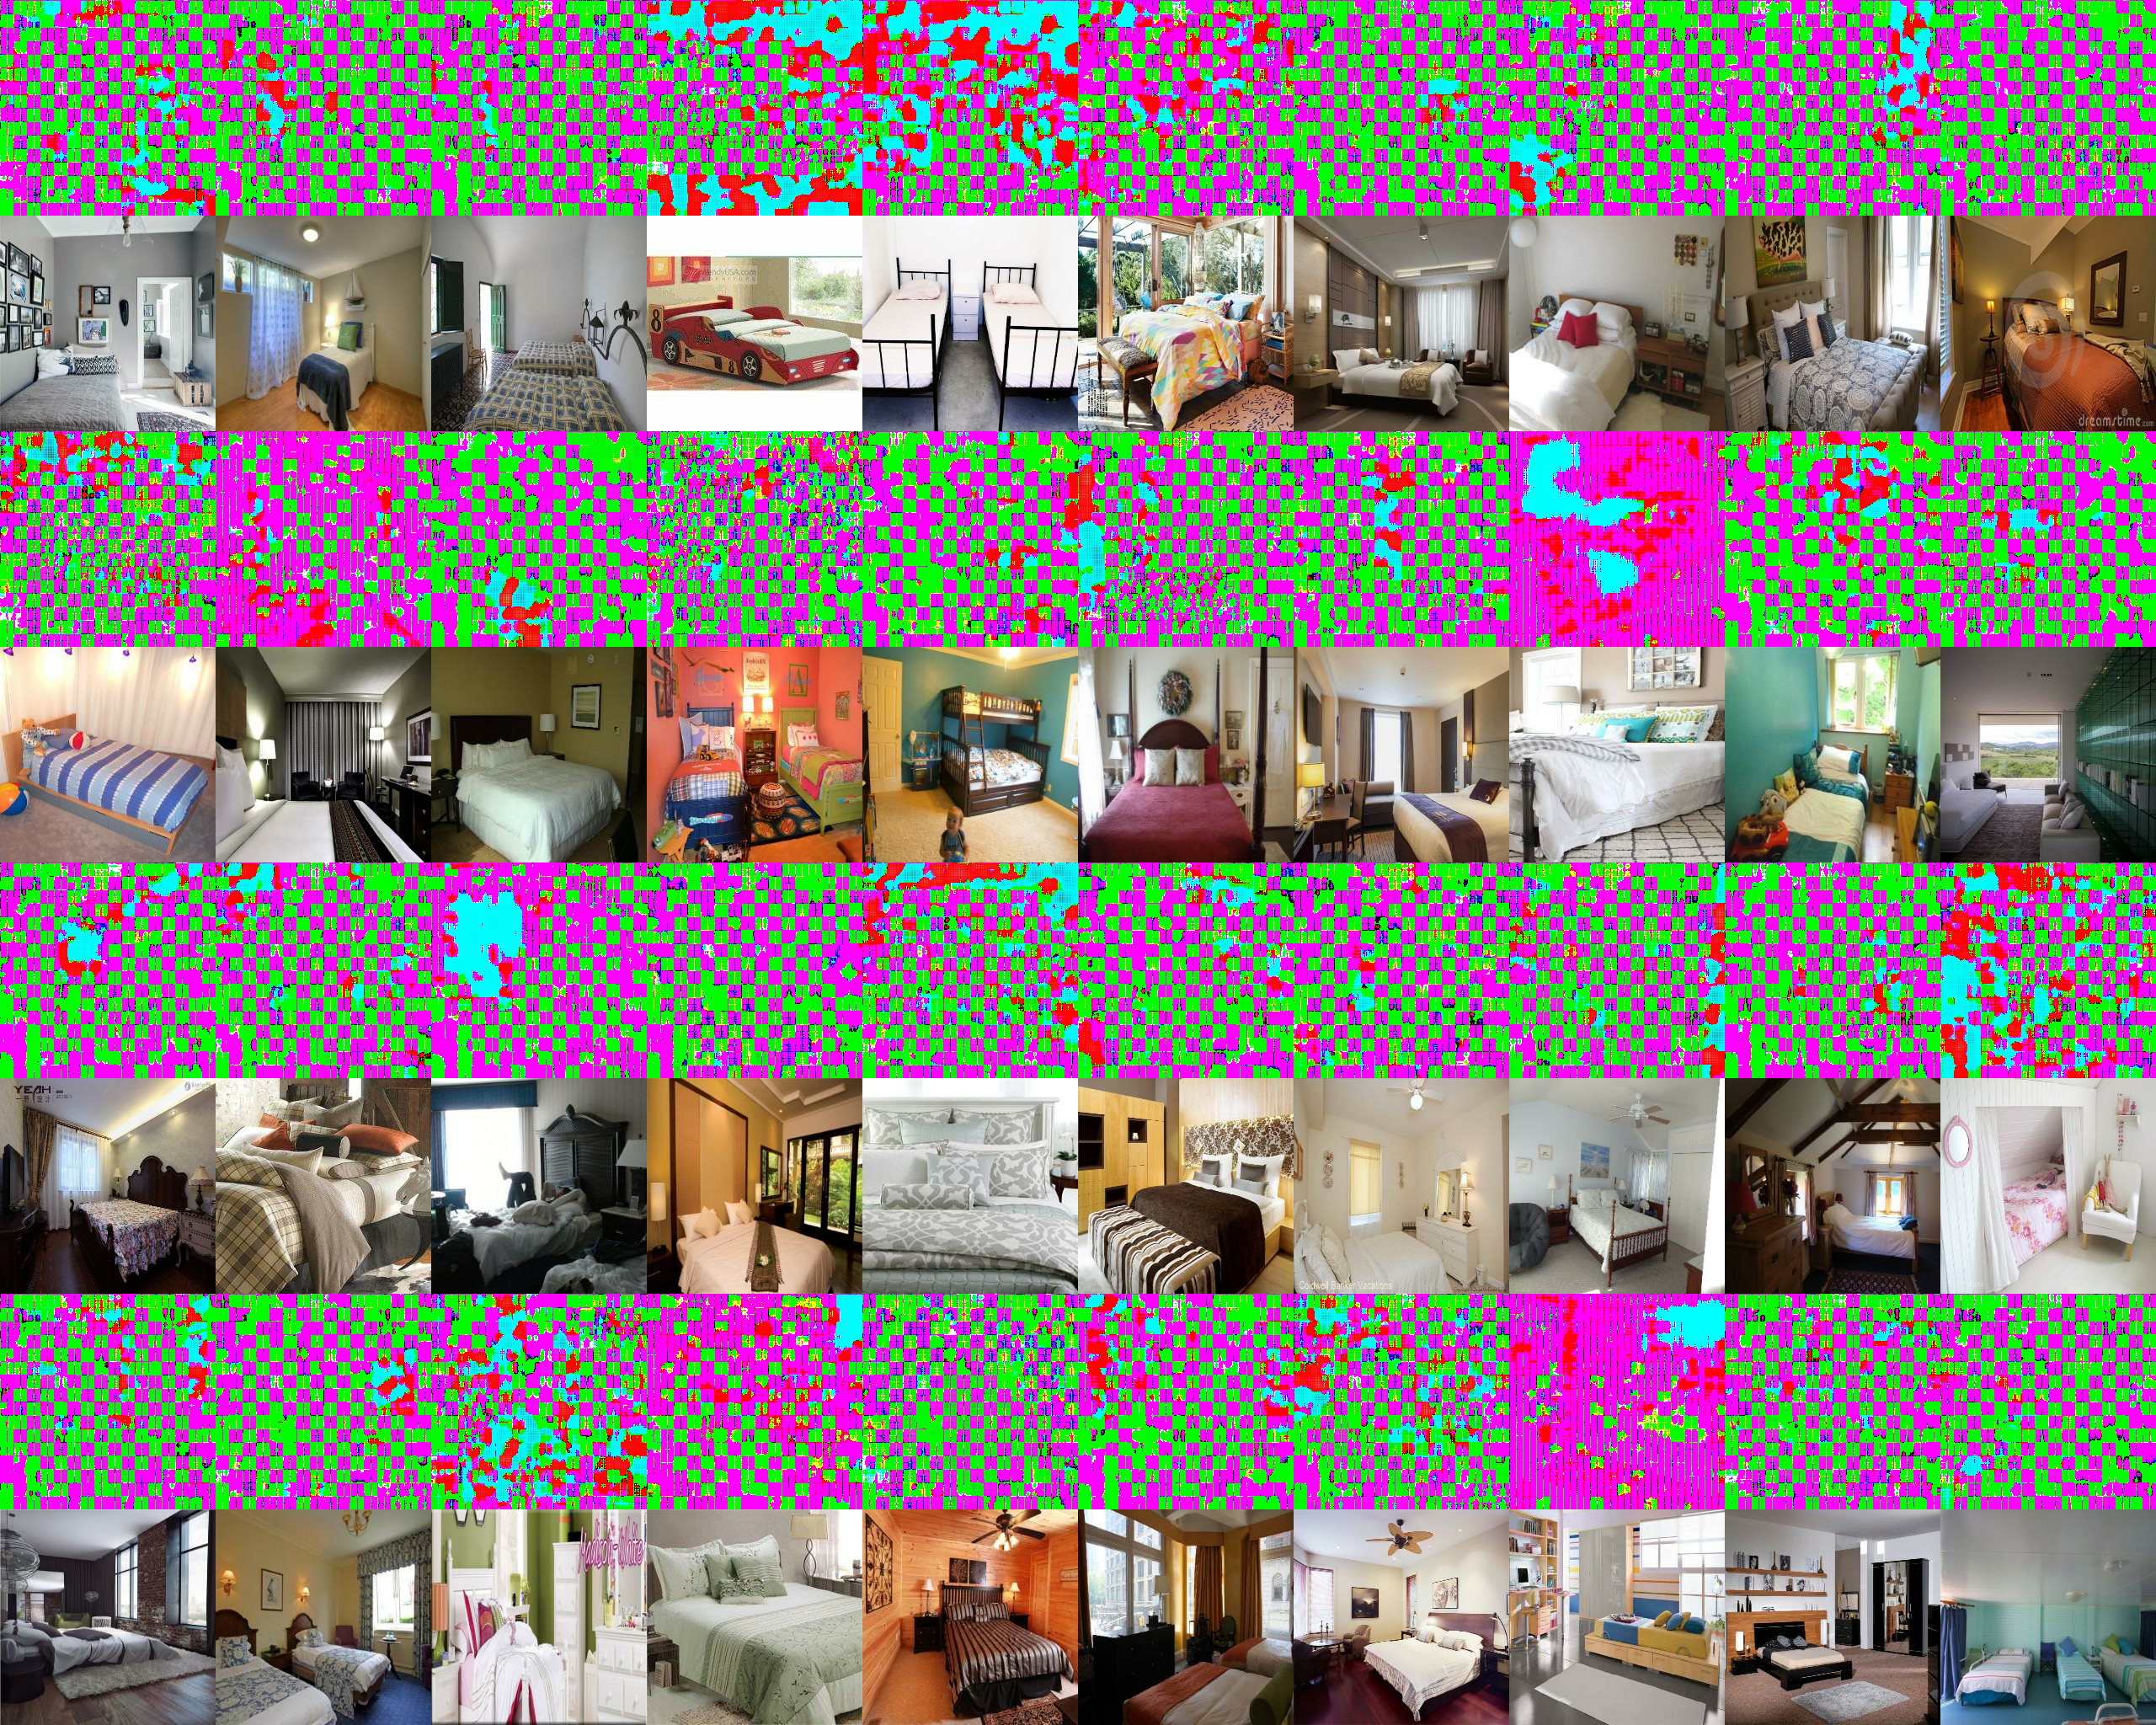
\includegraphics[scale=.95]{smoothgrad-big/combined_model/testing-3-2-combined-dataset-raw-smoothgrad.png}
          \caption{Real vs GAN classifier sensitivity - real image}
    \end{figure}
    
    \begin{figure}[H]
      \centering
        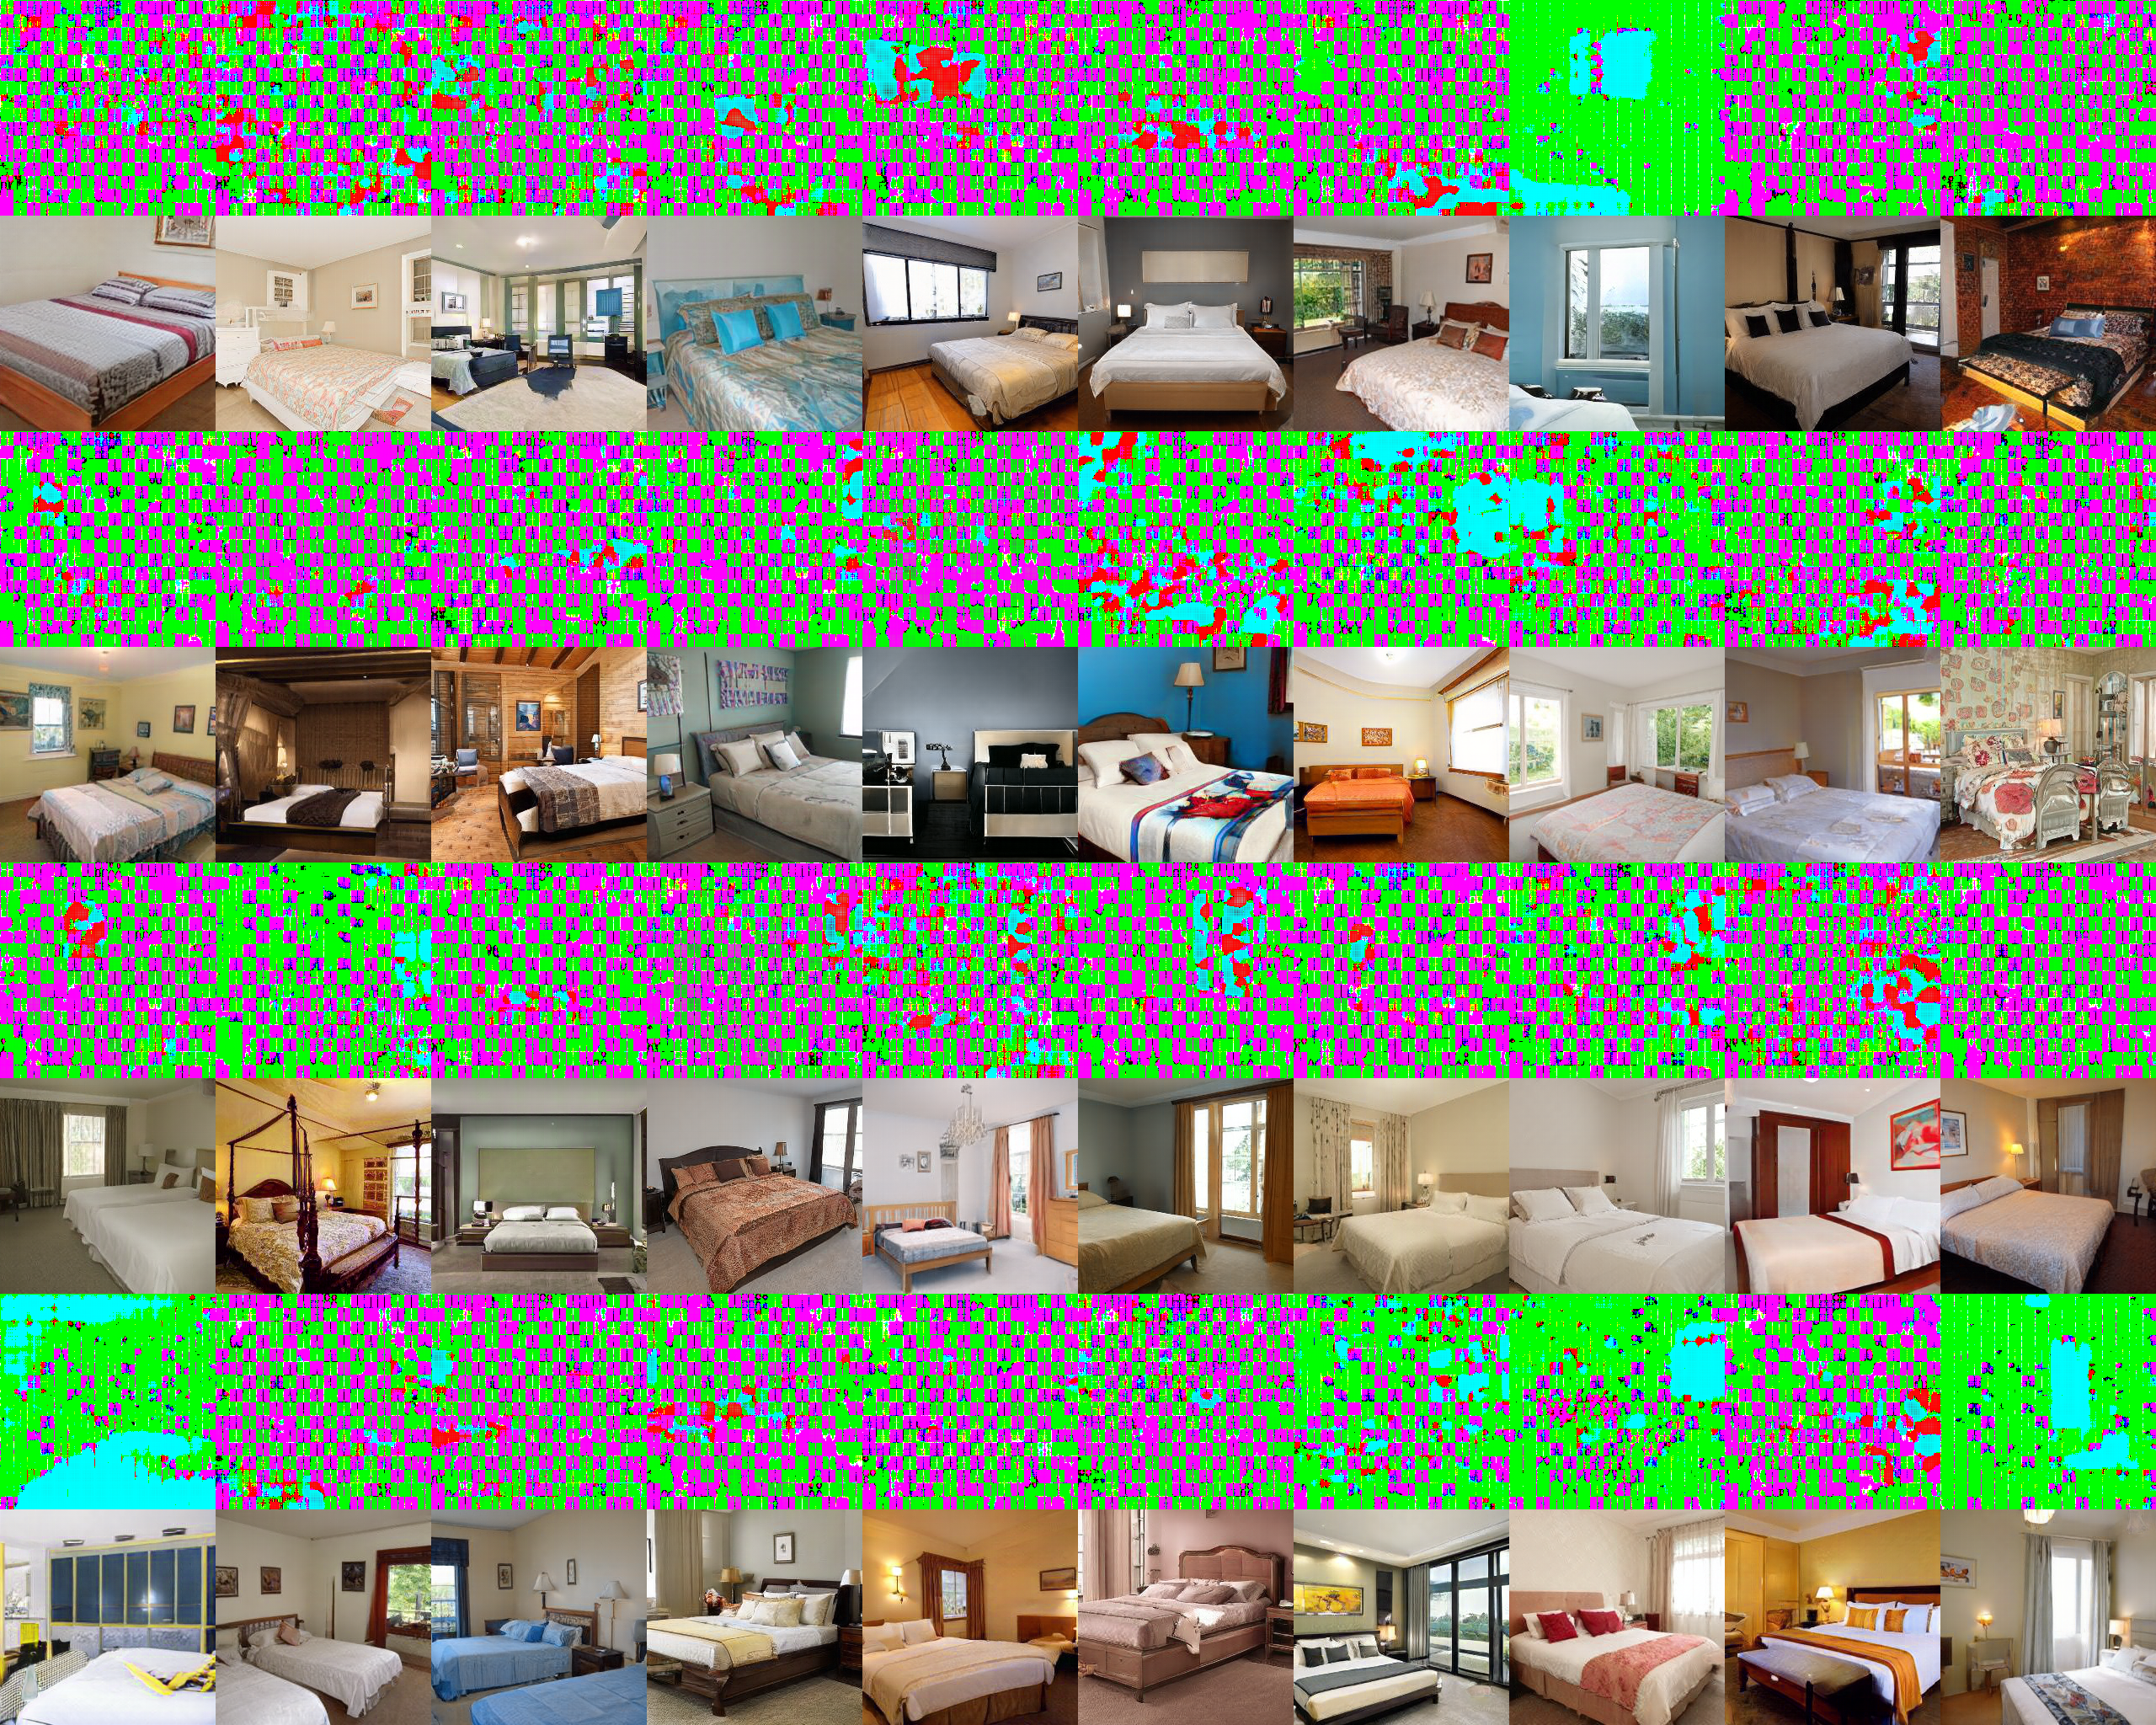
\includegraphics[scale=.95]{smoothgrad-big/combined_model/testing-3-2-combined-dataset-stylegan-smoothgrad.png}
     \caption{Real vs GAN classifier sensitivity - StyleGAN}
    \end{figure}
    
    \begin{figure}[H]
      \centering
        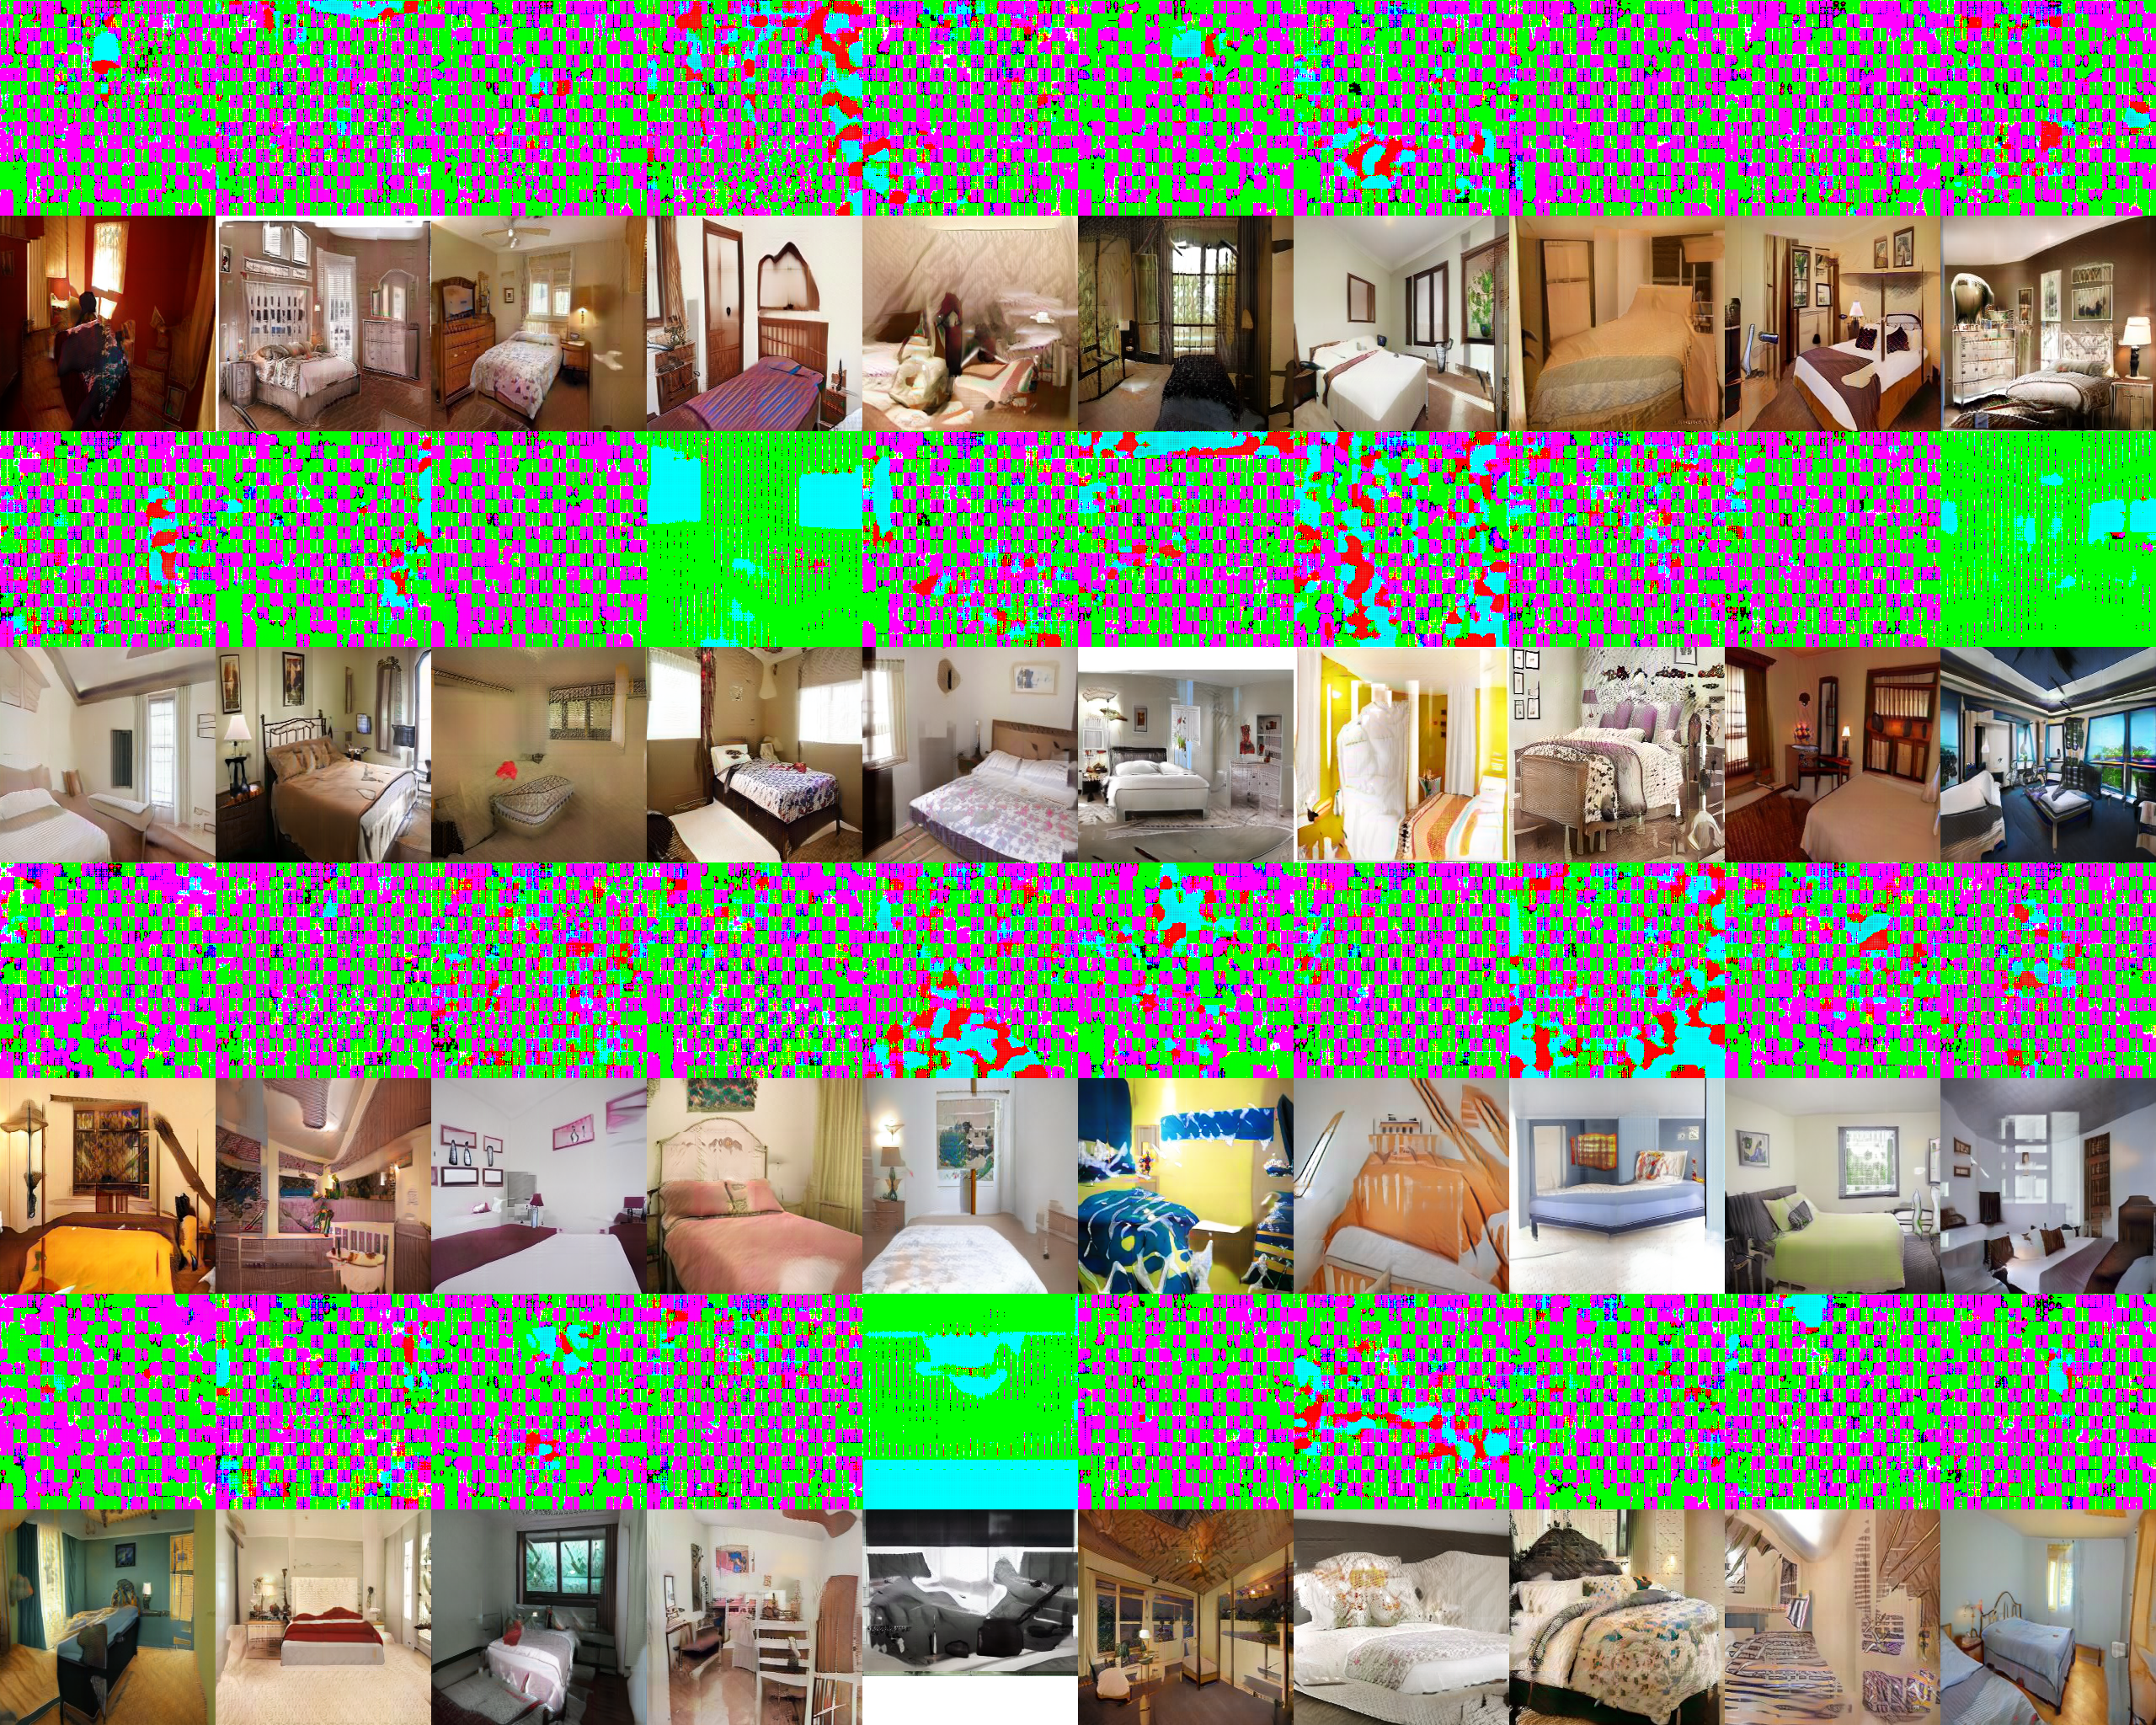
\includegraphics[scale=.95]{smoothgrad-big/combined_model/testing-3-2-combined-dataset-coco-smoothgrad.png}
      \caption{Real vs GAN classifier sensitivity - COCO-GAN}
    \end{figure}
       
    \begin{figure}[H]
      \centering
        \includegraphics[scale=.95]{smoothgrad-big/stylegan_model/testing-2-2-combined-dataset-raw-smoothgrad.png}  
        \caption{Real vs StyleGAN classifier sensitivity - real image}
    \end{figure}
    
    \begin{figure}[H]
      \centering
        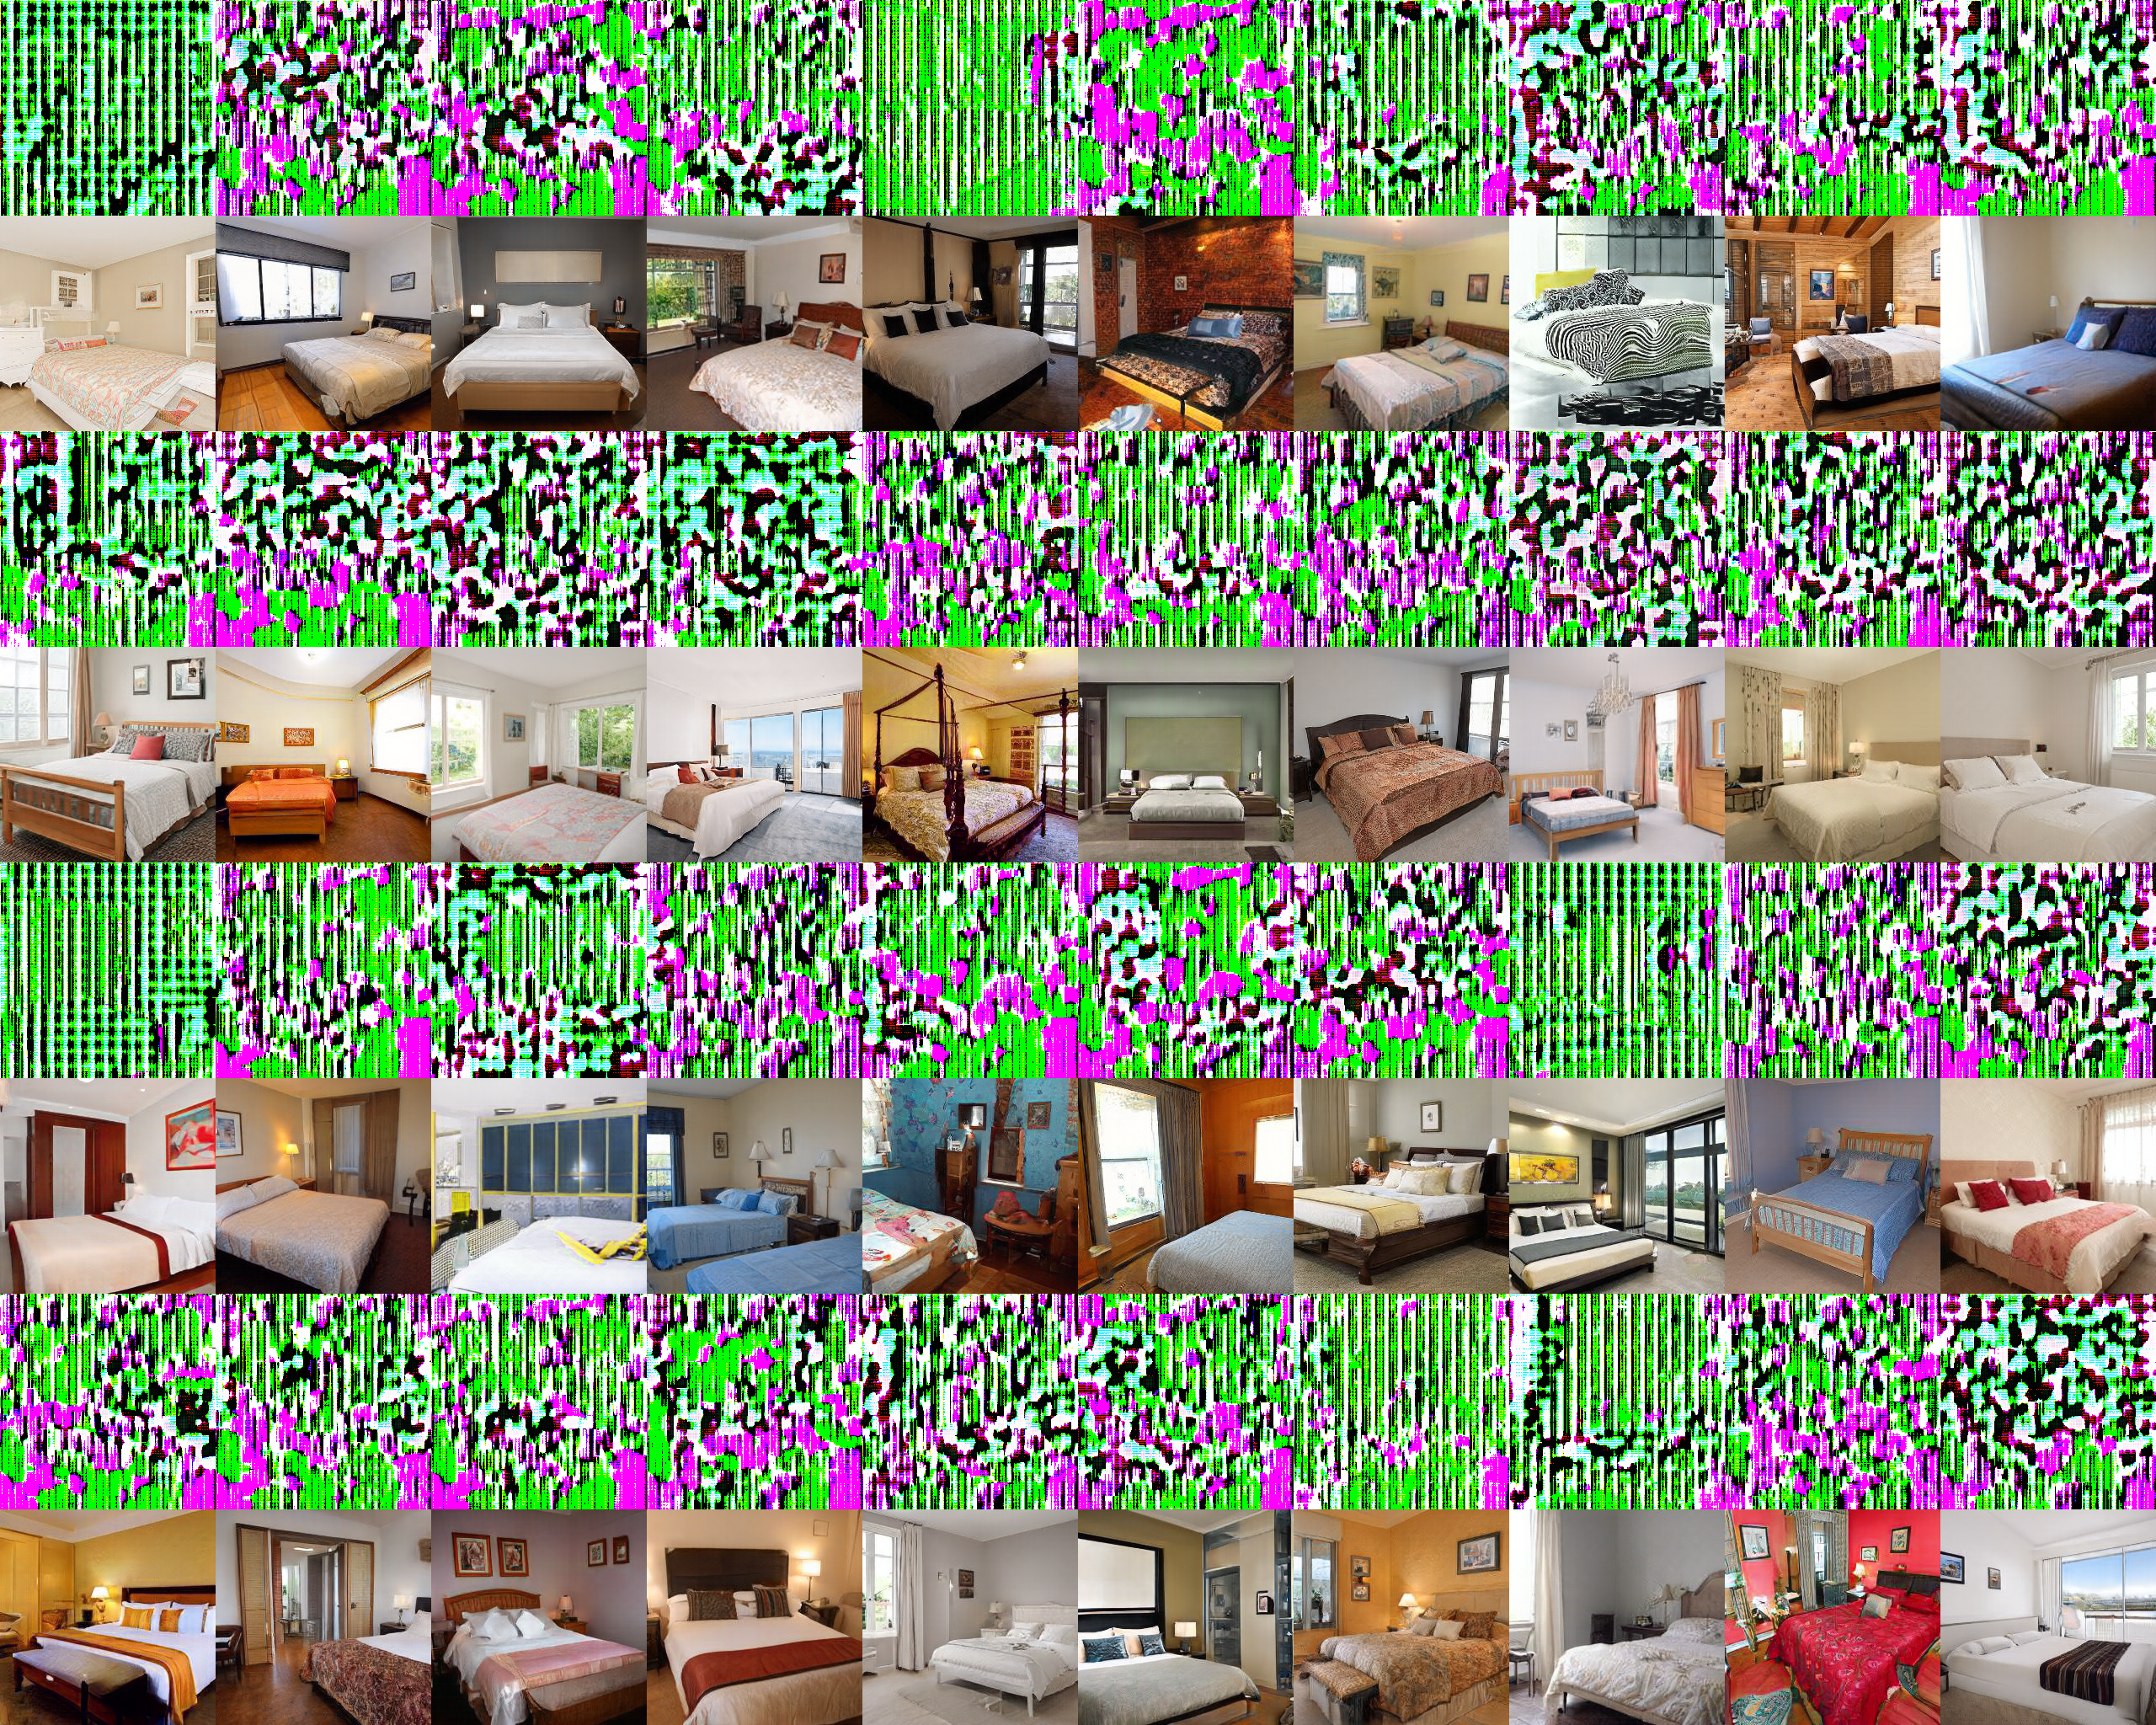
\includegraphics[scale=.95]{smoothgrad-big/stylegan_model/testing-2-2-combined-dataset-stylegan-smoothgrad.png}
        \caption{Real vs StyleGAN classifier sensitivity - StyleGAN}
    \end{figure}
    
    \begin{figure}[H]
      \centering
        \includegraphics[scale=.95]{smoothgrad-big/cocogan_model/testing-2-2-combined-dataset-raw-smoothgrad.png}
    \caption{Real vs COCO-GAN classifier sensitivity - real image}
    \end{figure}
    
    \begin{figure}[H]
      \centering
        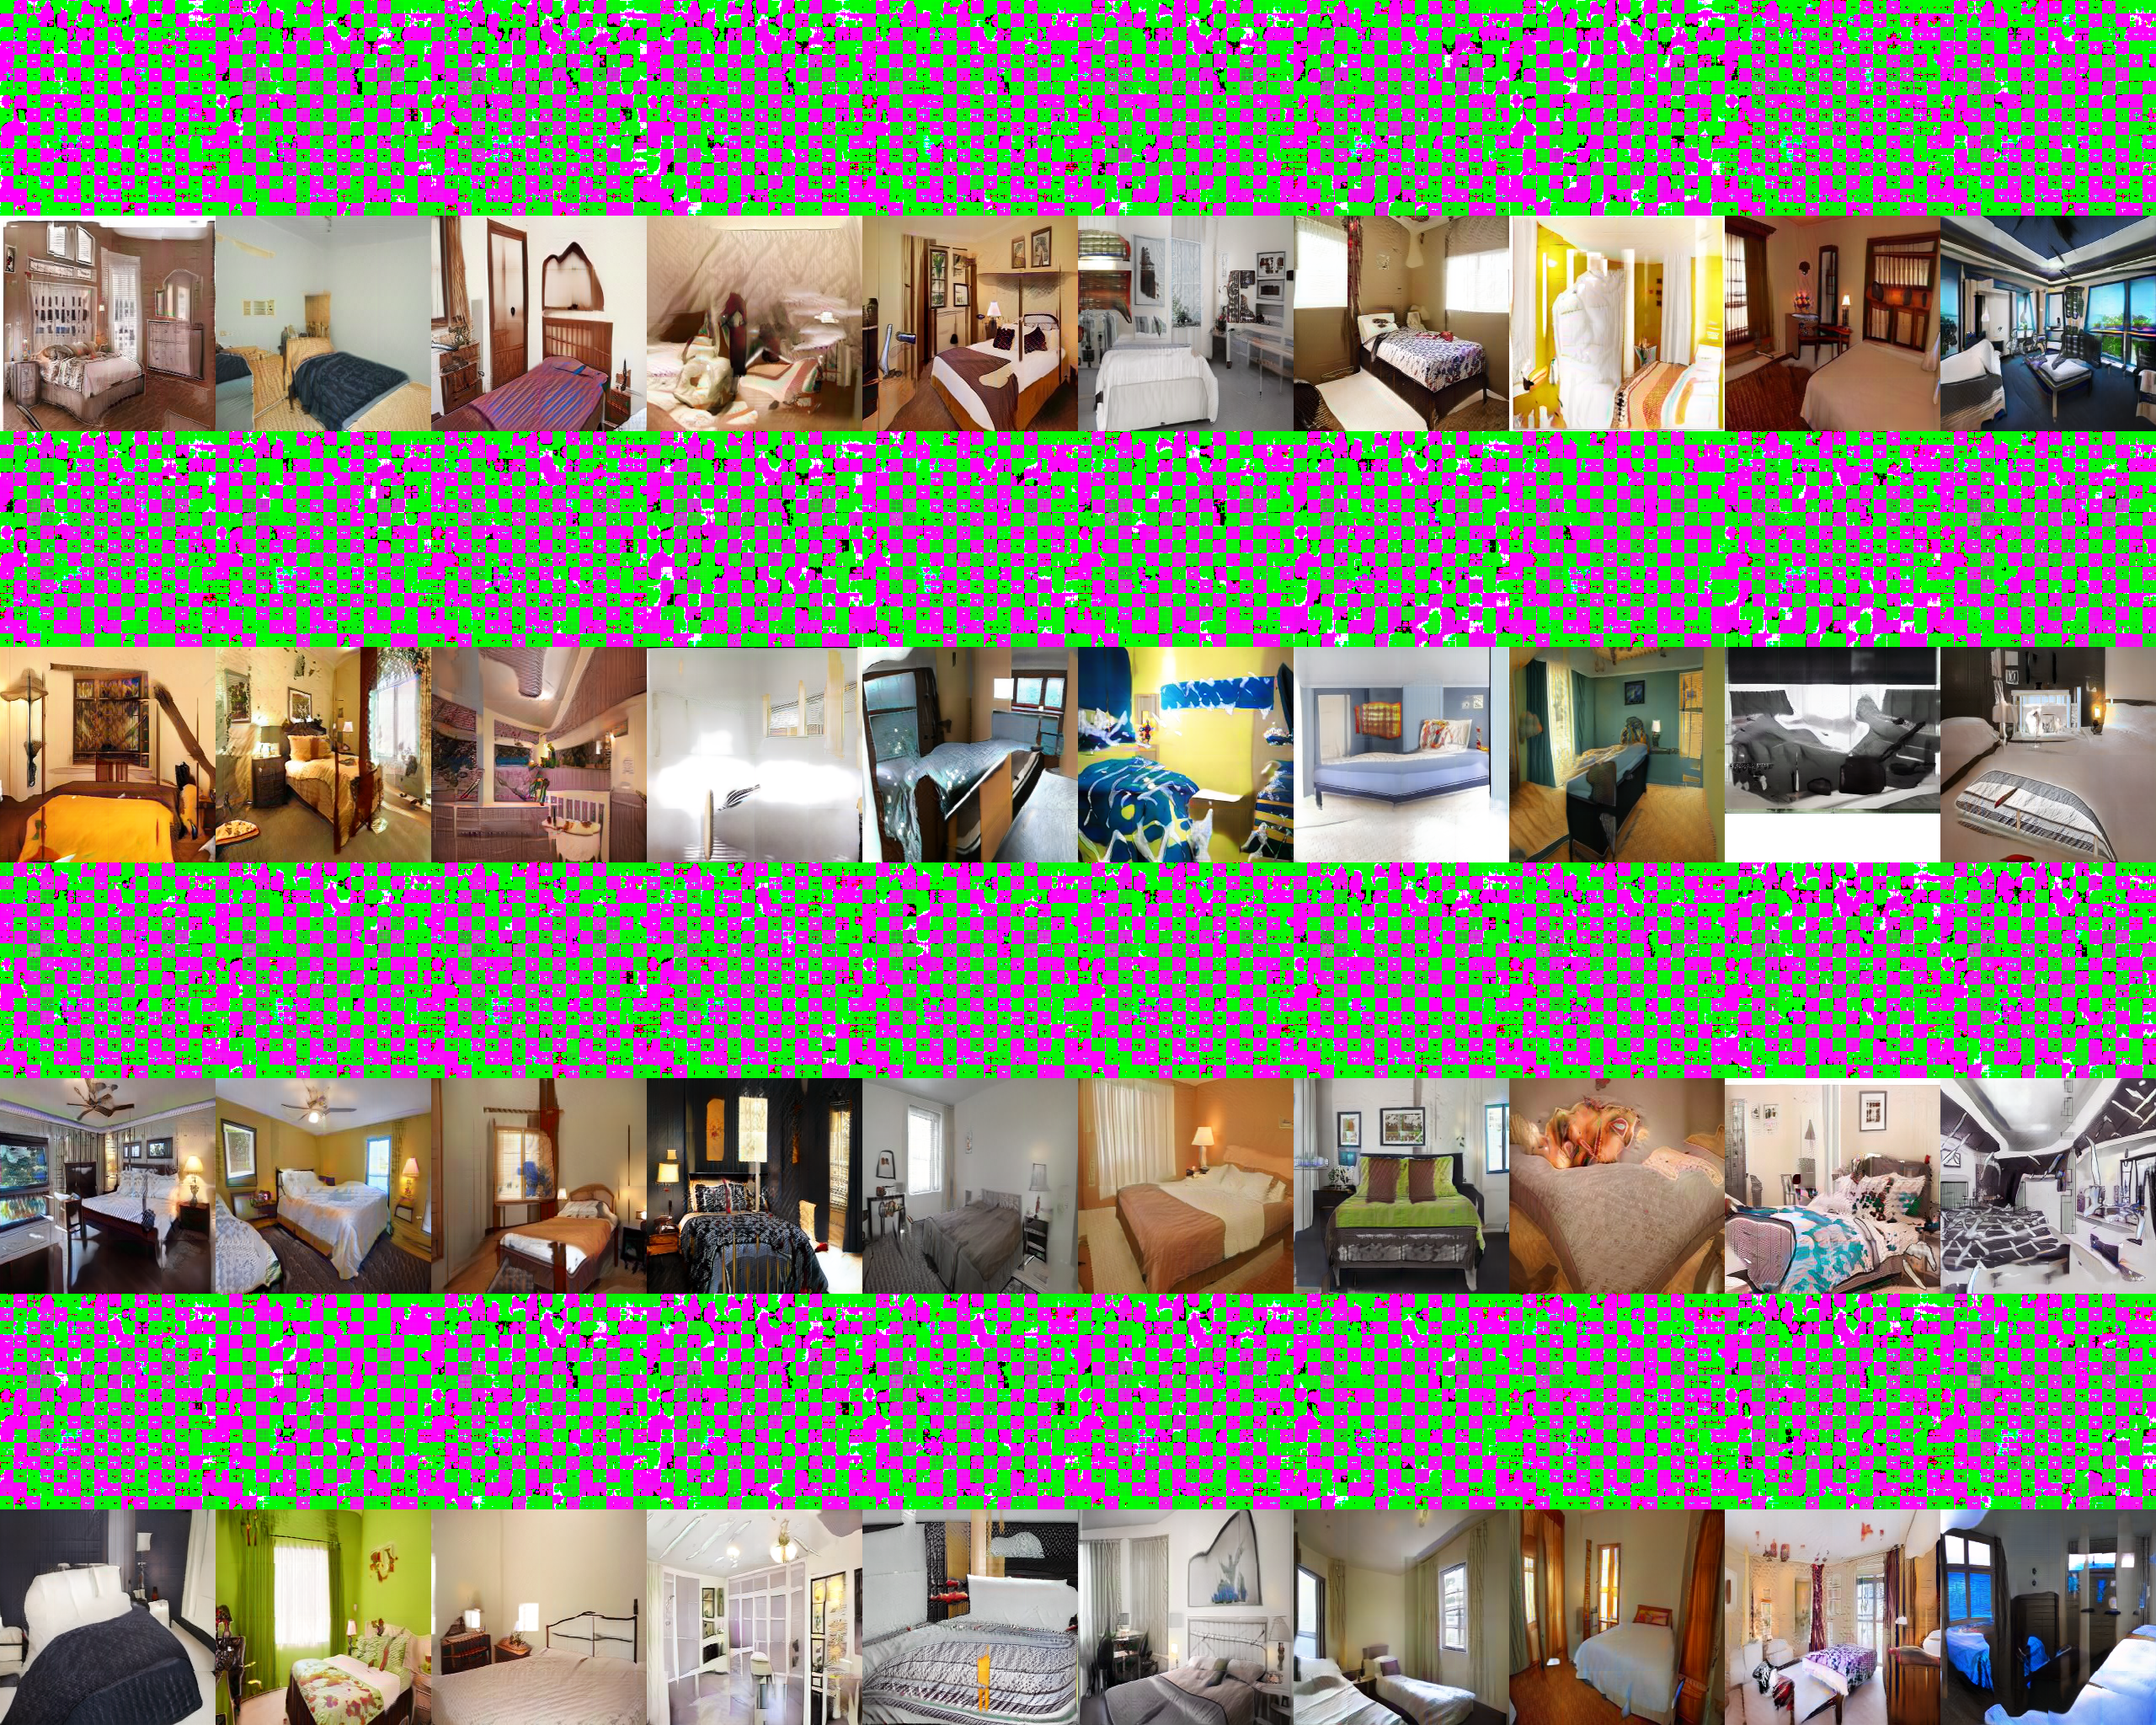
\includegraphics[scale=.95]{smoothgrad-big/cocogan_model/testing-2-2-combined-dataset-cocogan-smoothgrad.png}
    \caption{Real vs COCO-GAN classifier sensitivity - COCO-GAN}
    \end{figure}
    
\end{document}